\documentclass{beamer}
\usepackage{lmodern}
\usepackage{appendixnumberbeamer}
\renewcommand{\sfdefault}{lmss}
\renewcommand{\ttdefault}{lmtt}
\usepackage[T1]{fontenc}
% \usepackage[utf8]{inputenc}
\setcounter{secnumdepth}{3}
\setcounter{tocdepth}{3}
\usepackage{amsmath}
\usepackage{amsthm}
\usepackage{amssymb}
\theoremstyle{definition}
\newtheorem*{defn*}{\protect\definitionname}
\providecommand{\definitionname}{Definition}
\usepackage{graphicx}
\usepackage{hyperref}
\usepackage{ulem}
\PassOptionsToPackage{normalem}{ulem}
\usepackage{caption}
\usepackage{subcaption}
\usepackage{verbatim}
\usepackage[english]{babel}
\usepackage[autostyle]{csquotes}
\usepackage{tikz}
\usetikzlibrary{arrows,intersections}
\usepackage{pgfplots}
\pgfplotsset{compat = 1.15}
\usepgfplotslibrary{fillbetween}
\usepackage{verbatim}
\usepackage{booktabs}
\usepackage{multirow}
\usepackage{array}
\usepackage{nccmath}
% \usepackage{listings}
\usepackage{mathtools}

%Bibliography style, etc.
\usepackage[citestyle=authoryear-comp,natbib, uniquename = false, url = false, doi = false, uniquelist=false]{biblatex}
\renewbibmacro{in:}{}
\AtEveryBibitem{%
  \clearfield{volume}%
  \clearfield{number}
  \clearfield{month}
  \clearfield{issn}
  \clearfield{isbn}
  \clearfield{pages}
}

%\usepackage{cleveref}
\usepackage{setspace}
\makeatletter

% Macros
\providecommand{\tabularnewline}{\\}
\newcommand{\gr}{\textcolor{ForestGreen}} 
\newcommand{\rd}{\textcolor{red}}
\newcommand{\cb}{\textcolor{CornflowerBlue}} %this is the blue color you like; simply type \cb{X} where "X" is the color you want in blue
\newcommand{\vitem}{\vfill \item} %auto-centers items in lists
\newcommand{\fall}{\ \forall} %redefines "forall" (I don't like the default spacing)
\newcommand{\frall}{\quad \forall} %a \forall separated from the main math; this is the way it usually shows up in equations
\newcommand{\exist}{\ \exists} %same as \fall, but for \exists; they have the same ugly spacing
\newcommand{\R}{\mathbb{R}} %set of real numbers
\newcommand*\bigcdot{\mathpalette\bigcdot@{.5}} %different size for cdots
% \newcommand{\argmax}{\text{arg}\max}
\newenvironment{itemframe}
    {\frame{}\itemize}
    {\itemize\frame}
\newcommand\makebeamertitle{\frame{\maketitle}}%
\newtheoremstyle{named}{}{}{\itshape}{}{\bfseries}{.}{.5em}{\thmnote{#3's }#1}
\theoremstyle{named}
\newtheorem*{prop*}{Proposition}
% \newtheorem*{corollary}{Corollary}
\newtheorem*{namedtheorem}{Theorem} %allows named theorems
\newtheorem*{nameddef}{Definition}
\newtheorem{proposition}{Proposition}
\newtheorem*{assumption}{Assumption}
\newtheorem*{namedcorollary}{Corollary}
\newtheorem*{namedlemma}{Lemma}
\newtheorem*{axiom}{Axiom}
\newtheorem*{theorem*}{Theorem}
\newtheorem*{lemma*}{Lemma}
\DeclareMathOperator*{\argmin}{argmin}
\DeclareMathOperator{\argmax}{argmax}
\DeclareMathOperator{\supp}{supp}
\DeclareMathOperator{\interior}{int}
\DeclareMathOperator{\rank}{rank}
\newcolumntype{C}[1]{>{\centering\let\newline\\\arraybackslash\hspace{0pt}}m{#1}}
\newcommand{\sbt}{\,\begin{picture}(-1,1)(-1,-3)\circle*{2}\end{picture}\ }



%formatting
\usetheme{Ilmenau}
\definecolor{MIT}{rgb}{.639,.122,.204}
\definecolor{UCLA}{rgb}{0.15294117647058825, 0.4549019607843137, 0.6823529411764706}
\definecolor{UCLA_gold}{rgb}{1, 0.8196078431372549, 0}
\usecolortheme[named=UCLA]{structure}
\setbeamercolor*{palette secondary}{fg=UCLA_gold,bg=gray!15!white}
\usecolortheme{dolphin}
\setbeamertemplate{navigation symbols}{} 
\setbeamertemplate{footline}{}{}
\setbeamertemplate{headline}{}
\setbeamertemplate{navigation symbols}{}
\mode<presentation> {}
\setbeamercolor{block title}{use=structure,fg=white,bg=RoyalBlue} %blocks (theorems, etc.)in blue
\setbeamercolor{block title alerted}{use=structure,fg=white,bg=ForestGreen} %blocks (theorems, etc.)in blue

\renewcommand\qedsymbol{$\blacksquare$} %set QED symbol as black square
\renewcommand{\emph}{\textit} %set emphasized text style; this is italics
\setbeamertemplate{footline}[frame number] %slide numbers
\setbeamertemplate{itemize item}[circle] %bullet style
\setbeamertemplate{itemize subitem}{--}
\setbeamertemplate{enumerate item}[default]
\newrobustcmd*{\parentexttrack}[1]{%
  \begingroup
  \blx@blxinit
  \blx@setsfcodes
  \blx@bibopenparen#1\blx@bibcloseparen
  \endgroup}

\AtEveryCite{%
  \let\parentext=\parentexttrack%
  \let\bibopenparen=\bibopenbracket%
  \let\bibcloseparen=\bibclosebracket}

 \AtBeginDocument{%
   \let\origtableofcontents=\tableofcontents
   \def\tableofcontents{\@ifnextchar[{\origtableofcontents}{\gobbletableofcontents}}
   \def\gobbletableofcontents#1{\origtableofcontents}
 }
\newcommand{\backupbegin}{
   \newcounter{framenumberappendix}
   \setcounter{framenumberappendix}{\value{framenumber}}
}
\newcommand{\backupend}{
   \addtocounter{framenumberappendix}{-\value{framenumber}}
   \addtocounter{framenumber}{\value{framenumberappendix}} 
} 

\renewcommand{\maketitle}{
\setbeamertemplate{footline}{} 
\begin{frame}[noframenumbering]
\titlepage
\end{frame}
\setbeamertemplate{footline}[frame number]
}

\usefonttheme[onlymath]{serif}

% \usetheme{CambridgeUS}

% \newtheorem{theorem}{Theorem}
% \theoremstyle{claim}
\newtheorem{claim}{Claim}
% \newtheorem{corollary}{Corollary}


\makeatother


%\author{Drew Fudenberg}

\institute[]{}
\title{The Rise of Market Power and the Macroeconomic Implications}
\author{De Loecker, Eeckout, and Unger}

\begin{document}
\maketitle

\begin{frame}{Overview}
  \begin{itemize}
  \item Aggregate markups have risen from 21\% to 61\% since the 1980s
    \vitem \emph{Median} markups haven't changed
    \vitem The entire change in markup is due to a rise in markups for firms at the top of the markup distribution
    \vitem The authors show how to estimate these markups, document them robustly, and show that we care about the entire distribution of markups, not just a summary statistic
  \end{itemize}
\end{frame}
%
\begin{frame}{Estimating Markups}
  \begin{itemize}
  \item Existing approaches (BLP) rely on assumptions about consumer and firm behavior in order to get their results.
    \begin{itemize}
    \item BLP assumes firms compete via Nash-Bertrand and uses the FOC that comes out of that equation
    \end{itemize}
    \vitem \textbf{This paper:} estimates markup based on the wedge between an input's expenditure share (in revenue) and that input's output elasticity.
    \vitem Need to estimate a production function in order to do this.
  \end{itemize}
\end{frame}
%
\begin{frame}{Approach}
  \begin{itemize}
  \item Document some stylized facts about markups for the past 60 years.
    \vitem Show that these patterns are robust to different definitions of markups.
    \vitem \textbf{Question:} are markups rising exclusively because of increasing fixed costs?
    \vitem \textbf{Answer:} No; fixed costs have increased, but profit rates and markups have increased even more.
  \end{itemize}
\end{frame}
%
\begin{frame}{Production Function Approach to Markup Estimation}
\setlength{\jot}{20pt}
  \begin{align*}
    Q_{it} &= Q_{it}(\overbrace{\Omega_it}^{\mathclap{\text{productivity}}},\underbrace{V_{it}}_{\mathclap{\text{variable inputs}}}, K_{it}) \tag{production technology}\\
    \mathcal{L}(V_{it}, K_{it}, \lambda_{it}) &= P^V_{it}V_{it} + r_{it}K_{it} + F_{it} - \lambda_{it}(Q(\cdot) - \overline{Q}_{it})\\
    \frac{\partial \mathcal{L}}{\partial V_{it}} &= P_{it}^V - \lambda_{it} \frac{\partial Q(\cdot)}{\partial V_{}it} = 0 \tag{FOC}\\    \intertext{rearrange and multiply by $\frac{V_{it}}{Q_{it}}$ to get elasticity:}
    \theta_{it}^v &\equiv \frac{\partial Q(\cdot)}{\partial V_{it}}\frac{V_{it}}{Q_{it}}\\[-10pt]
    &= \frac{1}{\lambda_{it}} \frac{P_{it}^V}{Q_{it}}
  \end{align*}
\end{frame}
%
\begin{frame}{Production Function Approach to Markup Estimation}
  \begin{itemize}
  \item Does \rd{not} depend on specifying conduct or a particular demand system.
    \vitem In principle there are multiple FOCs that give an expression for markups
    \vitem Need two ingredients from the data:
    \begin{itemize}
    \item Revenue share of variable input, $\dfrac{P_{it}^V V_{it}}{P_{it}Q_{it}}$
      \vitem Output elasticity of the variable input, $\theta^v_{it}$
    \end{itemize}
  \end{itemize}
  \end{frame}
  %
  \begin{frame}{Data}
    \begin{itemize}
    \item Compustat Data for 60 years
      \vitem Construct user cost of capital as
      \[
r_t = (I_t - \Pi_t) + \Delta
      \]
      \vitem Use SG \&A as a measure of overhead
      \begin{itemize}
      \item Also consider a specification where overhead is a factor of production
      \end{itemize}
      \vitem Supplement Compustat data with Census data
    \end{itemize}
  \end{frame}
  %
  \begin{frame}{Evolution of Markups and Distribution of Markups}
    \begin{columns}
\begin{column}{0.5\textwidth}
     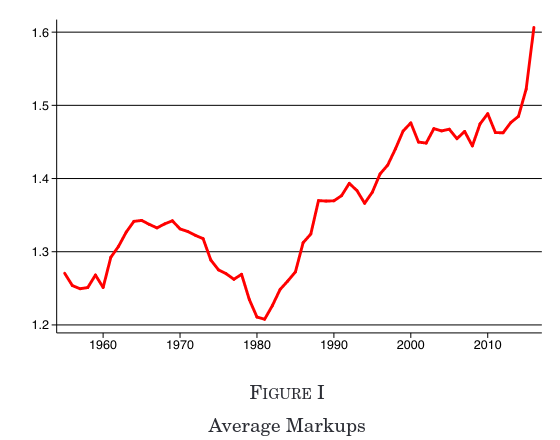
\includegraphics[width=\textwidth, keepaspectratio=true]{fig1.png}
\end{column}
\begin{column}{0.5\textwidth}  %%<--- here
    \begin{center}
     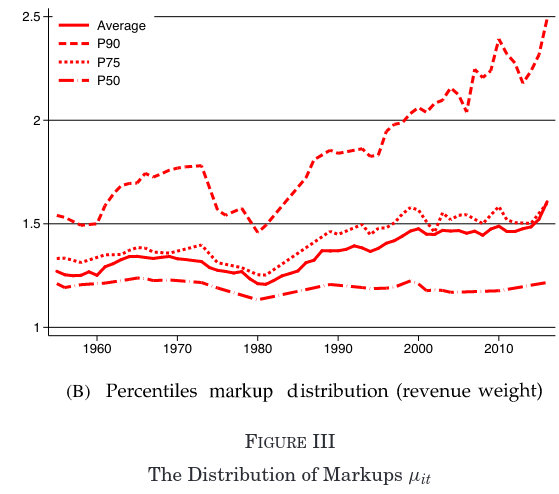
\includegraphics[width=\textwidth, keepaspectratio=true]{fig3.png}
     \end{center}
\end{column}
\end{columns}
  \end{frame}
  %
  \begin{frame}{Markup Growth at the Firm Level}
    There are two forces at work:
    \begin{enumerate}
    \item The markup (within term) increases
      \item Reallocation of sales to high-markup firms
    \end{enumerate}
    \begin{figure}[htp]
      \centering
      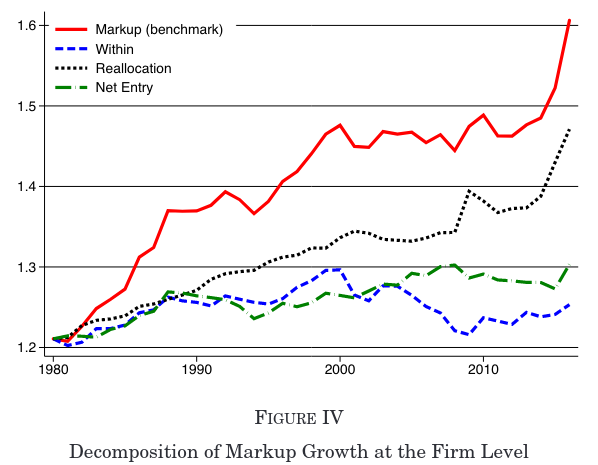
\includegraphics[width=0.8\textwidth, keepaspectratio=true]{fig4.png}
    \end{figure}
  \end{frame}
  %
  \begin{frame}{What do we lose when we use aggregate data?}
    \begin{columns}
\begin{column}{0.5\textwidth}
  \[\sum_i \frac{S_{it}}{P_{it}^V V_{it}} \ne \frac{\sum_i S_{it}}{\sum_i P^V_{it} V_{it}}\]
  \begin{itemize}
  \item The series based on aggregate data are all below the benchmark series
    \vitem A substantial part of the increase occurs within industry
    \vitem The dispersion and skewness of the distribution of markups have increased over time
  \end{itemize}
\end{column}
\begin{column}{0.65\textwidth}  %%<--- here
    \begin{center}
     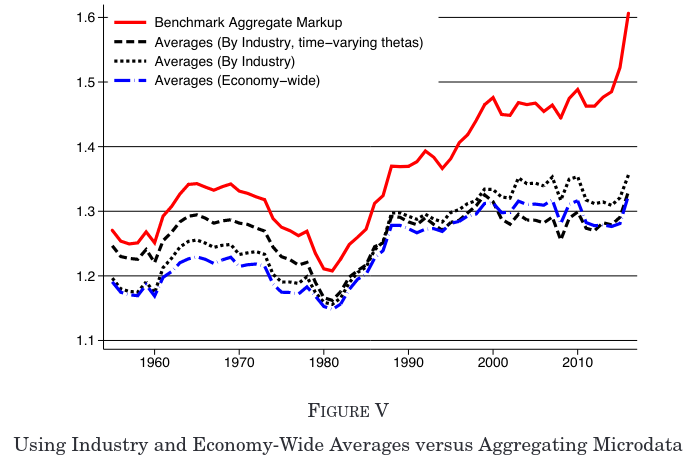
\includegraphics[width=\textwidth, keepaspectratio=true]{fig5.png}
     \end{center}
\end{column}
\end{columns}
  \end{frame}
  %
  \begin{frame}{Markups and Profits at the Firm Level}
    \begin{columns}
\begin{column}{0.5\textwidth}
  \[\pi_{it} = 1 - \frac{\theta_{st}}{\mu_{it}} - \frac{r_t K_{it}}{S_{it}} - \frac{P_t^X X_{it}}{S_{it}}\]
  \begin{itemize}
  \item This profit measure includes the output elasticity of the production technology
    \vitem The increase in average profits is almost exclusively driven by the increase in profits for high profit firms
  \end{itemize}
\end{column}
\begin{column}{0.5\textwidth}  %%<--- here
    \begin{center}
     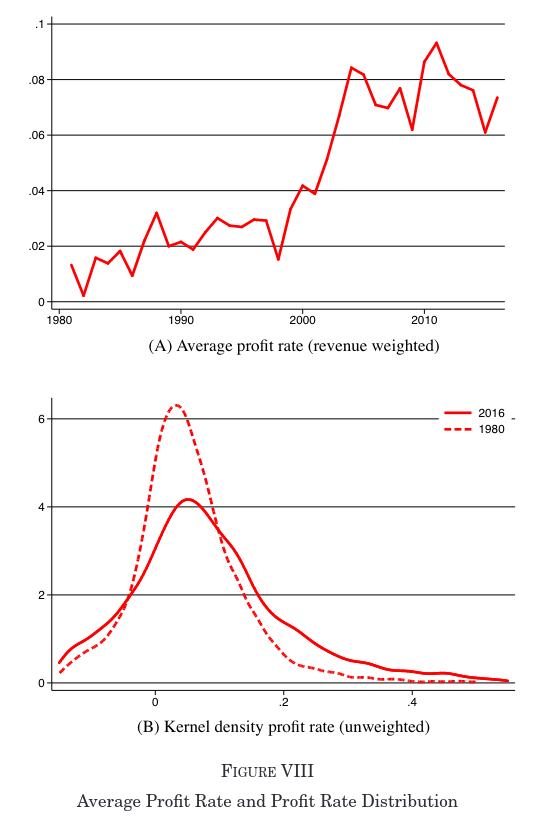
\includegraphics[width=\textwidth, keepaspectratio=true]{fig8.png}
     \end{center}
\end{column}
\end{columns}
  \end{frame}
  %
  \begin{frame}{Comparing Aggregate Profits and Markups}
    \[
\pi_{it} = \frac{P_{it} Q_{it} - C(Q_{it})}{P_{it} Q_{it}} = 1 - \frac{AC_{it}}{\mu_{it} MC_{it}} \tag{15}
    \] 
    \begin{itemize}
    \item Assuming constant ratio of $MC$ to $AC$ and representative firm, implied profit is 38\%. How to reconcile with the data?
    \end{itemize}
    \begin{figure}[htp]
      \centering
      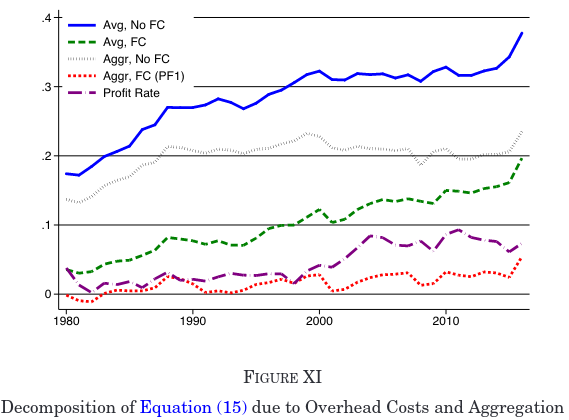
\includegraphics[width=0.7\textwidth, keepaspectratio=true]{fig15.png}
    \end{figure}
  \end{frame}
  %
  \begin{frame}{Conclusion}
    \begin{itemize}
    \item Since 1980, markups have risen from $21\% \to 61\%$, and profits from $1\% \to 8\%$
      \vitem Almost all the change is due to high-markup firms.
      \vitem The rise in markups is not simply offsetting increasing fixed costs (although fixed costs \emph{are} increasing).
      \vitem This provides one possible explanation for the secular decline in the labor share in the US.
    \end{itemize}
  \end{frame}
\end{document}
%%% Local Variables:
%%% mode: latex
%%% TeX-master: t
%%% End:
